% The roadmap: every part and lesson in build order, with what each lesson needs, its file, and how far it has got.
% Part numbers and lesson letters come from counters, so a lesson moved in this file is renumbered everywhere,
% the diagram included; chapters never carry them. Build with ./build.sh.

\documentclass[11pt,a4paper]{article}

\usepackage{fontspec}
\usepackage[margin=2.5cm]{geometry}
\usepackage{enumitem}
\usepackage{float}
\usepackage{chapter}
\usetikzlibrary{positioning}
\usepackage{hyperref}
\hypersetup{hidelinks}  % read on e-ink: references in plain black

\setlist[description]{style=nextline, leftmargin=1.5em}
\setlength{\parindent}{0pt}
\setlength{\parskip}{0.6em}

% A part is one new idea: \part{label}{title}{what it is about}. Its lessons are lettered:
% \lesson{label}{title}{file, or empty}{what it does}{what it needs}{built}{read}.
\newcounter{partno}
\setcounter{partno}{-1}
\newcounter{lesson}[partno]
\renewcommand{\thelesson}{\arabic{partno}\alph{lesson}}
\renewcommand{\part}[3]{\refstepcounter{partno}\label{#1}\section*{Part \thepartno: #2}#3}
\newcommand{\lesson}[7]{\refstepcounter{lesson}\label{#1}%
  \item[\thelesson. #2] #4\\
  \emph{Needs:} #5.\\
  \emph{File:} \if\relax\detokenize{#3}\relax none yet\else\name{#3}\fi.
  \emph{Built:} #6. \emph{Read:} #7.}

\title{Altair 8800 replica on a Tang Nano 9K\\[0.3em]\large Roadmap}
\author{}
\date{}

\begin{document}
\maketitle

The build is split into numbered parts, each with one new idea, and each part has lettered lessons. An arrow means that a part needs the one it comes from. Each lesson lists what it needs on the bench, its file, which is a standalone PDF, whether it is built, and whether its chapter has been read.

\begin{figure}[H]
  \centering
  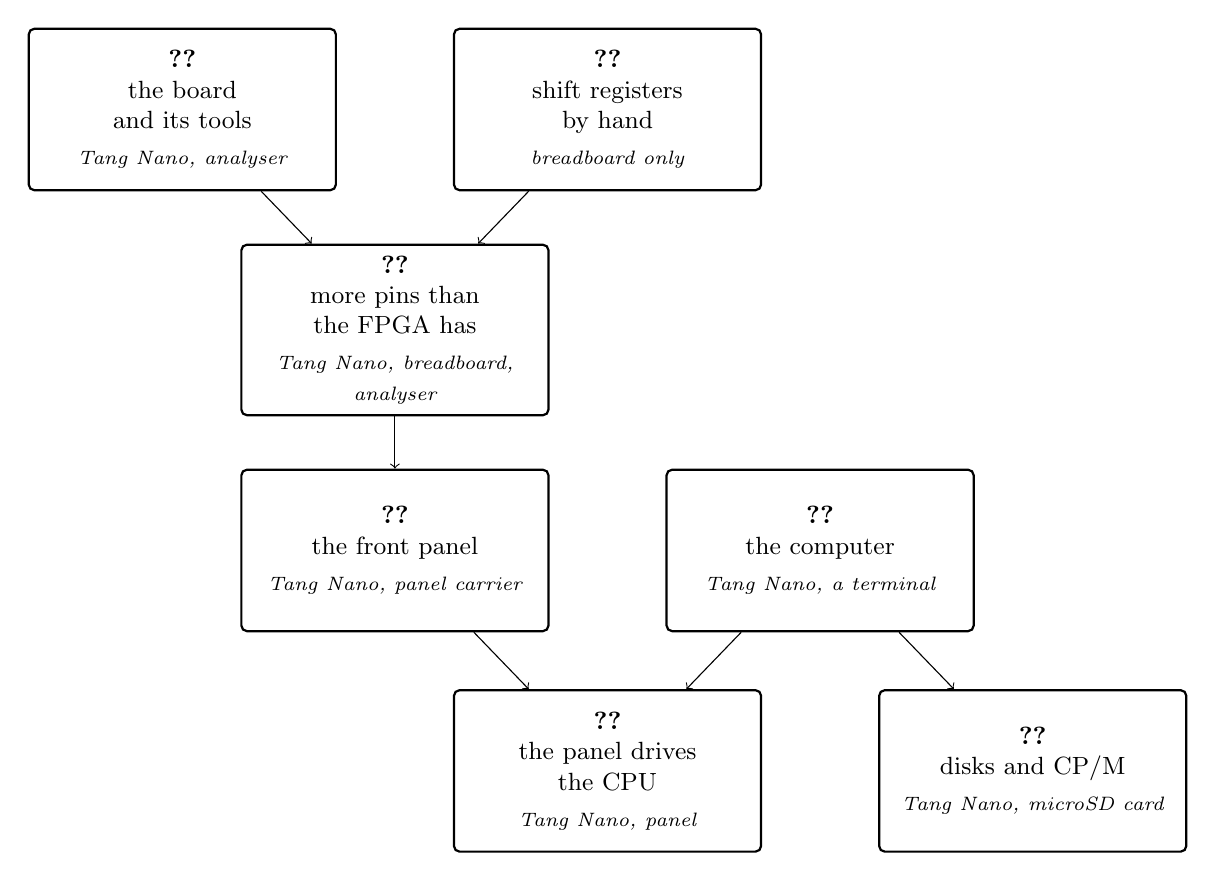
\begin{tikzpicture}[
      pt/.style={draw, thick, rounded corners=2pt, inner xsep=8pt, inner ysep=4pt, minimum width=3.9cm, minimum height=2.05cm, align=center, font=\small},
      needs/.style={font=\scriptsize\itshape},
      dep/.style={->}]
    \newcommand{\ptbox}[3]{\textbf{\ref{#1}}\\#2\\[2pt]\scriptsize\itshape #3}
    \node[pt] (p0) at (0, 0)      {\ptbox{pt:board}{the board\\and its tools}{Tang Nano, analyser}};
    \node[pt] (p1) at (5.4, 0)    {\ptbox{pt:byhand}{shift registers\\by hand}{breadboard only}};
    \node[pt] (p2) at (2.7, -2.8) {\ptbox{pt:shift}{more pins than\\the FPGA has}{Tang Nano, breadboard,\\\scriptsize\itshape analyser}};
    \node[pt] (p3) at (2.7, -5.6)   {\ptbox{pt:panel}{the front panel}{Tang Nano, panel carrier}};
    \node[pt] (p4) at (8.1, -5.6)   {\ptbox{pt:cpu}{the computer}{Tang Nano, a terminal}};
    \node[pt] (p5) at (5.4, -8.4) {\ptbox{pt:front}{the panel drives\\the CPU}{Tang Nano, panel}};
    \node[pt] (p6) at (10.8, -8.4){\ptbox{pt:disks}{disks and CP/M}{Tang Nano, microSD card}};
    \foreach \a/\b in {p0/p2, p1/p2, p2/p3, p3/p5, p4/p5, p4/p6} \draw[dep] (\a) -- (\b);
  \end{tikzpicture}
\end{figure}

\part{pt:board}{the board and its tools}{This part covers the Tang Nano 9K, the two ways of programming it, and the logic analyser that checks what it sends.}

\begin{description}
  \lesson{ls:leds}{Running LEDs, with Gowin EDA and the open-source flow}{running-leds.pdf}
    {The old LED project is rebuilt in Gowin EDA, step by step, and then the same two files go through the open-source flow, from a \name{Makefile}. The lessons after this one use the open flow.}
    {Tang Nano 9K}{yes}{yes}
  \lesson{ls:factory}{The factory program}{factory.pdf}
    {This lesson shows what the board runs out of the box and why it can’t be copied, and it writes the design that puts it back after a \texttt{make flash}.}
    {Tang Nano 9K}{yes}{yes}
  \lesson{ls:hello}{Hello world on the logic analyser}{hello-analyser.pdf}
    {A Verilog UART sends ‘Hello world’, and both the logic analyser’s decoder and a serial terminal read it back. This checks the analyser on a known signal.}
    {Tang Nano 9K on the breadboard, logic analyser}{no}{no}
\end{description}

\part{pt:byhand}{shift registers by hand}{Buttons drive the two shift registers, before any FPGA, and do by hand what the FPGA does later.}

\begin{description}
  \lesson{ls:595hand}{One \name{74HC595} by hand}{595-by-hand.pdf}
    {This lesson converts serial to parallel. Three buttons shift a byte in, bit by bit, and then latch it onto eight LEDs.}
    {breadboard, power module, \name{74HC595}, three buttons, eight LEDs}{yes}{yes}
  \lesson{ls:165hand}{One \name{74HC165} by hand}{165-by-hand.pdf}
    {This lesson converts parallel to serial. Eight switches load at once, and then a button clocks them out, one by one, onto a single LED.}
    {breadboard, power module, \name{74HC165}, 8-way DIP switch, buttons, one LED}{no}{no}
\end{description}

\part{pt:shift}{more pins than the FPGA has}{The FPGA takes the place of the buttons. Three pins drive eight outputs through the \name{74HC595}, three more read eight inputs through the \name{74HC165}, and chaining adds more of each. Timing is counted in clock cycles.}

\begin{description}
  \lesson{ls:walk}{A walking bit on the \name{74HC595}}{595-by-fpga.pdf}
    {One lit LED walks forward a bit at a time, and then backward a byte at a time. Both designs run in simulation first.}
    {Tang Nano 9K, the \name{74HC595} breadboard, logic analyser}{no}{in review}
  \lesson{ls:counter}{A byte counter on the \name{74HC595}}{}
    {The eight LEDs count in binary, with a whole byte written and latched on each tick.}
    {Tang Nano 9K, the \name{74HC595} breadboard, logic analyser}{no}{---}
  \lesson{ls:165}{Reading switches with a \name{74HC165}}{}
    {The FPGA loads the switches, shifts their eight bits in, and mirrors them on the \name{595}’s LEDs. A debounce module samples them at about 1\,kHz.}
    {Tang Nano 9K, both breadboards, logic analyser}{no}{---}
  \lesson{ls:chain}{A chain of two}{}
    {A second \name{595} and a second \name{165} are each fed by the first, so 16 switches are mirrored on 16 LEDs, and the width is a parameter.}
    {Tang Nano 9K, a second \name{74HC595} and \name{74HC165}}{no}{---}
\end{description}

\part{pt:panel}{the front panel}{Every toggle and LED of the Altair’s panel sits on a perfboard carrier.}

\begin{description}
  \lesson{ls:panelio}{The full panel interface}{}
    {Five \name{595}s and four \name{165}s sit behind one \texttt{panel\_io} module, with \texttt{led[35:0]} and \texttt{sw[31:0]}.}
    {Tang Nano 9K, perfboard carrier, toggles, and LEDs}{no}{---}
\end{description}

\part{pt:cpu}{the computer}{An 8080 runs the Altair’s software and talks through a terminal.}

\begin{description}
  \lesson{ls:core}{CPU and memory}{}
    {An 8080 core runs at 2\,MHz, with block RAM and ROM, and the Altair serial board is mapped to the USB-serial bridge. Altair 4K BASIC runs on a serial terminal.}
    {Tang Nano 9K, a serial terminal on the Mac}{no}{---}
  \lesson{ls:lcd}{LCD terminal}{}
    {The Sipeed 5-inch LCD works as an 80-column text terminal and shows what the serial terminal shows.}
    {Tang Nano 9K, Sipeed 5-inch LCD}{no}{---}
\end{description}

\part{pt:front}{the panel drives the CPU}{The front panel’s switches and lights are wired to the running machine.}

\begin{description}
  \lesson{ls:frontlogic}{Front panel logic}{}
    {The address and data LEDs show the live bus, and STOP, SINGLE STEP, EXAMINE, and DEPOSIT work. Kill the Bit is toggled in by hand and played.}
    {Tang Nano 9K, the panel}{no}{---}
\end{description}

\part{pt:disks}{disks and CP/M (optional)}{The Altair’s floppy drives live on the microSD card.}

\begin{description}
  \lesson{ls:cpm}{Disks and CP/M}{}
    {The floppy controller is emulated on the microSD card, and CP/M 2.2 boots.}
    {Tang Nano 9K, microSD card}{no}{---}
\end{description}

\section*{Schematics}

\begin{itemize}
  \item The \name{74HC595} and \name{74HC165} at flip-flop level: \name{74hc595-74hc165-internals.pdf}
  \item First byte, one byte in and one byte out: \name{altair-first-byte-schematic.pdf}
  \item Panel: \name{altair-panel-sr-schematic.pdf}
\end{itemize}

The parts list is \name{docs/parts.md} in the repo.

\end{document}
